\documentclass[11pt]{article}

\usepackage{graphicx}
%\usepackage{algorithmic}
%\usepackage{algorithm}
\usepackage{amssymb}
\usepackage{amsmath}
\usepackage{enumerate}
\usepackage[mathscr]{euscript}

\begin{document}

\pagenumbering{arabic}

\begin{center}
{\LARGE{\textbf{Affective Computing}}} \\
\Large\textsc{Ph.D. Comprehensive Exam} \\[1em]
\large\textnormal{Mohammad Shayganfar - mshayganfar@wpi.edu} \\
\large\textnormal{May, 26 2015}
\end{center}

\section{Introduction to Affective Computing}
According to Picard \cite{picard:affective-computing}, the term affective
computing encapsulates a new approach in Artificial Intelligence, to build
computers that show human affection. Studies show that the decision making of
humans is not always logical \cite{GrossbergGutowski:affect-cognition}, and in
fact, not only is pure logic not enough to model human intelligence, but it also
shows failures when applied in artificial intelligence systems
\cite{dreyfus:artificial-critique}. Emotions impact fundamental parts of
cognition including perception, memory, attention and reasoning
\cite{clore:judgement-regulation}. This impact is caused by the information
emotions carry about the environment and event values.

If we want robots and virtual agents to be more believable and efficient
partners for humans, we must consider the personal and social functionalities
and characteristics of emotions; this will enable our robots to coexist with
humans, who are emotional beings. To have a better understanding of applications
of affective computing, we can categorize the whole existing literature of
computational emotion modeling and their applications into four major categories
of: a) detecting and recognizing human emotions, b) interpreting and
understanding human emotions, c) generating artificial emotions and applying the
underlying processes to exploit emotion functions, and d) expressing
human-perceivable emotions during interaction.

There are some major emotion theories including \textit{appraisal, dimensional}
and \textit{discrete (basic)} theories, some of which have corresponding
computational models, e.g., EMA \cite{marsella:ema-process-model} and WASABI
\cite{becker:wasabi,becker:wasabi-description}. These models have been used in
different domains including AI and robotics. Modeling and applying these
theories can help robots and virtual agents to achieve communicative,
evaluative, interpretive, and regulatory aspects of emotions in some or all of
the four application domains we mentioned above.

This document provides description of major computational emotion theories,
their comparison, and their applications in AI and robotics. It includes the
existing influential computational emotion theories as well as the underlying
psychological theories; it majorly focuses on appraisal and dimensional
theories, although it briefly mentions other approaches, e.g. discrete (basic)
emotions.

\section{Computational Theories of Emotion/Affect}
\label{sec:emotion-theories}

There are different types of computational theories of emotion. These theories
differ in the type of relationships between their components and whether a
particular component plays a crucial role in an individual emotion. For
instance, the basic component of an emotion can be the behavioral tendencies,
the cognitive elements, or the somatic processes. Emotion theories can also
differ based on their representationial distinction.

\subsection{Appraisal Theory}
\label{sec:appraisal-theory}

Appraisal theories of emotion were first formulated by Arnold
\cite{arnold:emotion-personality} and Lazarus \cite{lazarus:emotion-adaptation}
and then were actively developed in the early 80s by Ellsworth and Scherer and
their students \cite{roseman:appraisal-theory}
\cite{sander:systems-approach-appraisal} \cite{scherer:nature-function-emotion}
\cite{scherer:emotions-emergent} \cite{scherer:appraisal-processes}. The
emotional experience is the experience of a particular situation
\cite{frijda:emotions}. Appraisal theory describes the cognitive process by
which an individual evaluates the situation in the environment with respect to
the individual's well-being and triggers emotions to control internal changes
and external actions.

\begin{figure}[tbh]
  \center
  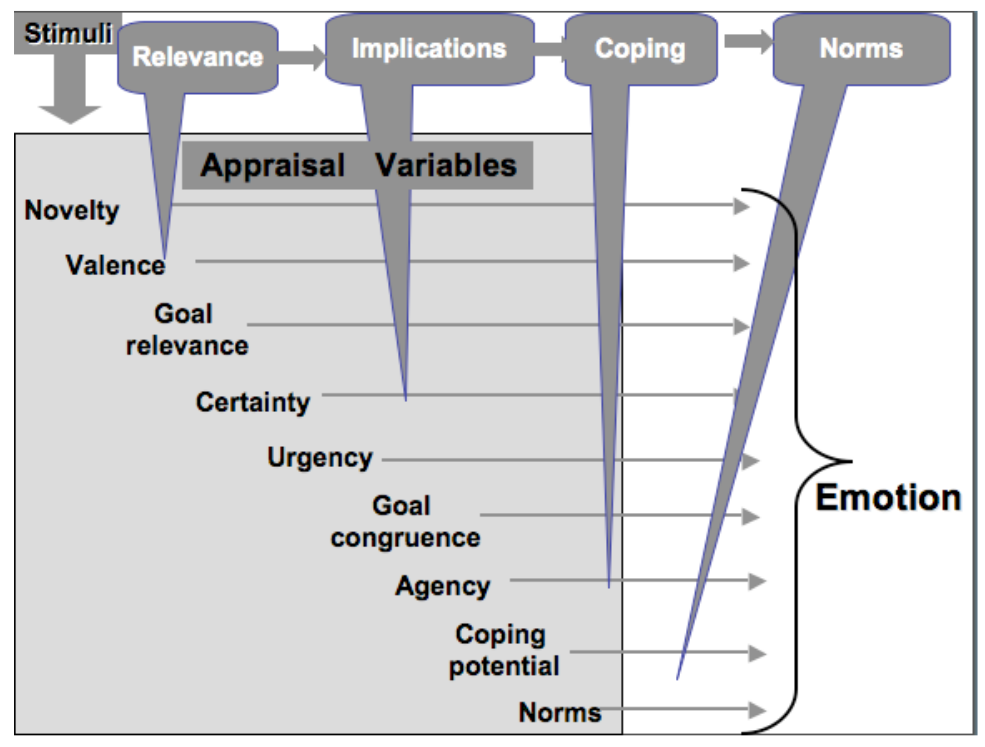
\includegraphics[width=0.8\textwidth]{figure/cpm.png}
  \caption{Schematic view of the componential theory of emotion
  \cite{hudlicka:guidelines-emotions}.}
  \label{fig:cpm}
\end{figure}

\subsubsection{Componential Approach}
\label{sec:componential-theories}

This approach emphasizes the distinct components of emotions, and is often
called the \textit{componential} approach \cite{leventhal:emotion-cognition}.
The ``components" referred to in this approach are the components of the
cognitive appraisal process. These are referred to as \textit{appraisal
variables}, and include \textit{novelty, valence, goal relevance, goal
congruence}, and \textit{coping abilities}
(further on, in this section, some of the appraisal variables used in
computational models are introduced)
\cite{scherer:nature-function-emotion,scherer:appraisal-processes}. A stimulus,
whether real or imagined, is analyzed in terms of its meaning and consequences
for the agent, to determine the affective reaction. The analysis involves
assigning specific values to the appraisal variables. Once the appraisal
variable values are determined by the organism’s evaluative processes, the
resulting vector is mapped onto a particular emotion, within the n-dimensional
space defined by the n appraisal variables. The semantic primitives for
representing emotions within this model are thus these individual appraisal
variables. Figure \ref{fig:cpm} shows the relationship of the individual
appraisal dimensions to the broader categories of evaluations taking place
during appraisal (Relevance, Implications, etc.).

\subsubsection{Component Process Model}
\label{sec:cpm}

The Component Process Model (CPM) is Scherer's influential and major theory of
emotions
\cite{scherer:sequential-appraisal-process,scherer:appraisal-processes}. This
theory focuses on the dynamic unfolding of emotions. The CPM suggests that an
event and its consequences are appraised with a set of criteria on multiple
levels of processing (the appraisal component). The result of the appraisal will
generally have a motivational effect, often changing or modifying the
motivational state before the occurrence of the event. Based on the appraisal
results and the motivational changes, some effects will occur in the autonomic
and somatic nervous system. The CPM considers emotions as the synchronisation of
many different cognitive and physiological components. Emotions are identified
with the overall process whereby low level cognitive appraisals, in particular
the processing of relevance, trigger bodily reactions, behaviours and subjective
feelings. The model suggests that there are four major appraisal objectives
required to adaptively react to a salient event
\cite{scherer:dynamic-architecture-emotion}:

\begin{enumerate}[a)]
  \item \textbf{Relevance:} How relevant is this event for the agent? Does it
  directly affect the agent or its social reference group?
  \item \textbf{Implications:} What are the implications or consequences of this
  event and how do they affect agent's well-being and its immediate or long-term
  goals?
  \item \textbf{Coping Potential:} How well can the agent cope with or adjust to
  these consequences?
  \item \textbf{Normative Significance:} What is the significance of this event
  for the agent's self-concept and for social norms and values?
\end{enumerate}

To attain these objectives, the agent evaluates the event and its consequences
on a number of criteria or \textit{Stimulus Evaluation Checks} (SECs), with the
results reflecting the agent’s subjective assessment of consequences and
implications on a background of personal needs, goals, and values
\cite{scherer:appraisal-processes}. Figure \ref{fig:comp-cpm} shows the
postulated sequence, the cognitive and motivational inputs and the effects on
response systems. Also, the bidirectional effects between appraisal and other
cognitive functions are illustrated by the arrows in the upper part of Figure
\ref{fig:comp-cpm}.

\begin{figure}[tbh]
  \center
  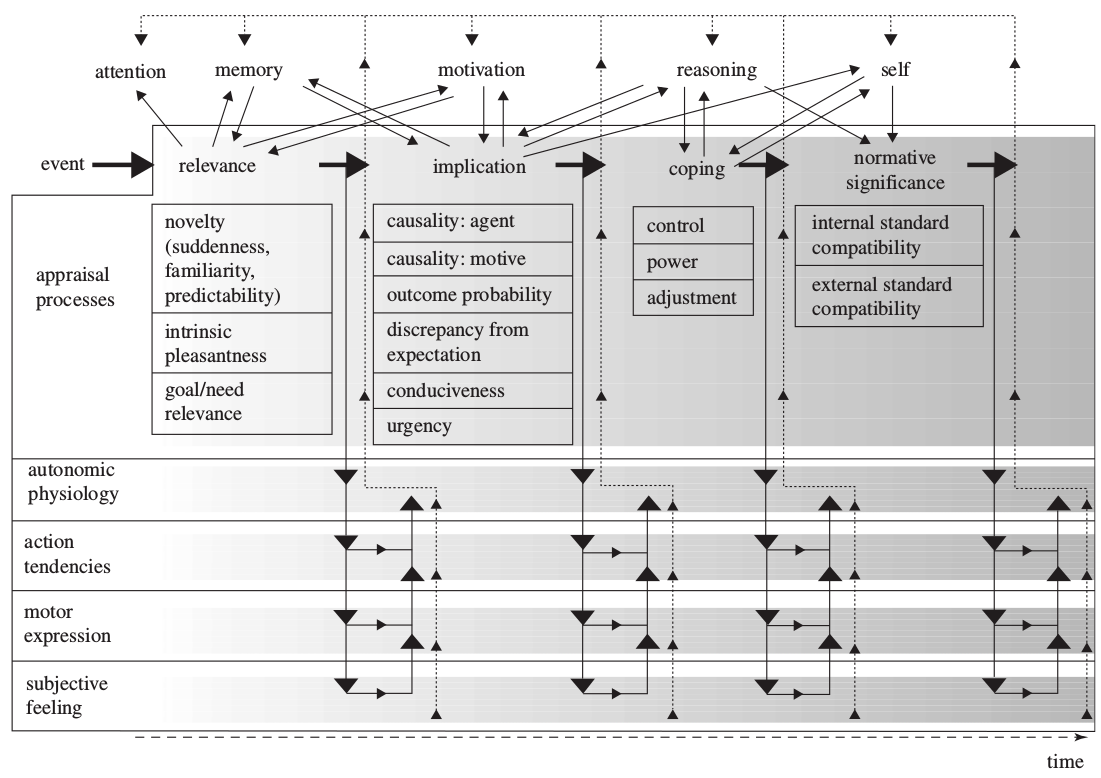
\includegraphics[width=\textwidth]{figure/comprehensive-CPM.png}
  \caption{Comprehensive illustration of the CPM of emotion
  \cite{scherer:dynamic-architecture-emotion,scherer:appraisal-processes}.}
  \label{fig:comp-cpm}
\end{figure}

\subsubsection{Appraisal Process}
\label{sec:appraisal-process}

According to this theory, appraisals are separable antecedents of emotion, that
is, the individual first evaluates the environment and then feels an appropriate
emotion \cite{scherer:appraisal-processes}. The appraisal procedure begins with
the evaluation of the environment according to the internalized goals and is
based on systematic assessment of several elements
\cite{scherer:sequential-appraisal-process}. The outcome of this process
triggers the appropriate emotions. In many versions of appraisal theory,
appraisals also trigger cognitive responses often called \textit{coping
strategies}. In fact, the coping mechanism manages the individual's action with
respect to the individual's emotional state and the existing internal and/or
external demands \cite{folkman:coping-pitfalls-promise}. The large majority of
computational models of emotions are based on this theory. An individual can
also use knowledge about the emotional reactions of others to make inferences
about them. According to the appraisal patterns, different emotions can be
experienced and expressed. Since expression of emotions reflects one's
intentions through the appraisal process, the \textit{reverse appraisal}
mechanism helps one to infer others' mental states based on their expressions.
\cite{gratch:reverse-appraisal, hareli:emotional-reaction-perception}.

Appraisal process is typically viewed as the cause of emotion and the cognitive
and behavioral changes associated with emotion. For instance, a particular
pattern of the appraisal variables (i.e., individual judgements) will elicit a
certain emotion or emotional expressions. These appraisal variables include
\cite{marsella:ema-process-model}:\\

\begin{itemize}
  \item \textbf{Relevance:} A relevant event has non-zero utility for an agent.
  This relevancy can either be based on a negative influence of an event on the
  agent or a positive one.
  
  \item \textbf{Perspective:} The point of view in which an event will be
  judged, e.g. self or other.
  
  \item \textbf{Desirability:} A desirable event advances a state of the utility
  for an agent whose perspective is being taken, or if it is an
  undesirable event, inhibits that.
  
  \item \textbf{Likelihood:} A measure of likelihood of the outcome.
  
  \item \textbf{Expectedness:} The extent to which the truth value of a state
  could have been predicted from causal interpretation.
  
  \item \textbf{Causal Attribution:} The agent who deserves the credit/blame.
  
  \item \textbf{Controllability:} Whether the outcome can be altered by the
  agent whose perspective is taken (this variable is related to the coping
  process).
  
  \item \textbf{Changeability:} Whether the outcome can be altered by some other
  causal agent (this variable is related to coping process).
\end{itemize}

\subsubsection{Coping Process}
\label{sec:coping-process}

Another key process involved in appraisal is the coping process. This process
determines whether and how the agent shoud respond with respect to the outcome
of appraising the events. There are several coping strategies that computational
models like EMA \cite{gratch:domain-independent} use as control signals. These
control signals enable or suppress the cognitive processes that operate on the
causal interpretation of the appraisal patterns. The coping process controls the
congruency of the actions according to these patterns. As it is shown below, in
\cite{gratch:domain-independent} coping strategies are organized into two
categories: \textit{problem-focused} and \textit{emotion-focused}.
Problem-focused coping strategies can be applied when the agent must do
something with respect to the problem, whereas Emotion-focused coping works by
changing one's interpretation of circumstances. The following is a short list of
a broad range of coping strategies \cite{gratch:domain-independent}:

\begin{description}
  \item[Problem-focused coping] \hfill
	\begin{itemize}
	  \item \textbf{Active coping:} Taking active steps to remove or circumvent the
	  stressor,
	  \item \textbf{Planning:} Coming up w/ action strategies,
	  \item \textbf{Seeking social support for instrumental reasons:} Seeking
	  advice, assistance, or information.
	\end{itemize}
  \item[Emotion-focused coping] \hfill
    \begin{itemize}
	  \item \textbf{Seeking social support for instrumental reasons:} Getting
	  sympathy, moral support or understanding,
	  \item \textbf{Acceptance:} Accepting the stressor and learning to live with
	  it,
	  \item \textbf{Restraint coping:} Waiting till the appropriate opportunity
	  (holding back).
	\end{itemize}
\end{description}

\subsubsection{OCC, a Structural Appraisal Theory of Emotion}

OCC (Ortony, Clore and Collins) model, similar to Lazarus'
\cite{lazarus:cognitive-theory-emotion} and Scherer's
\cite{scherer:nature-function-emotion} cognitive views, considers emotions to
arise from affective or valenced reactions subsequent to the appraisal of a
stimulus as being beneficial or harmful to one’s concern \cite{occ:structure}.
The model categorizes emotions based on their underlying appraisal patterns.
These patterns are fundamental criteria a person employs for evaluating a
situation. They involve the person's focus of attention, her concern, and
her appraisal preceding an affective reaction. Figure \ref{fig:occ-model} shows
main building blocks of OCC model.

\begin{figure}[tbh]
  \center
  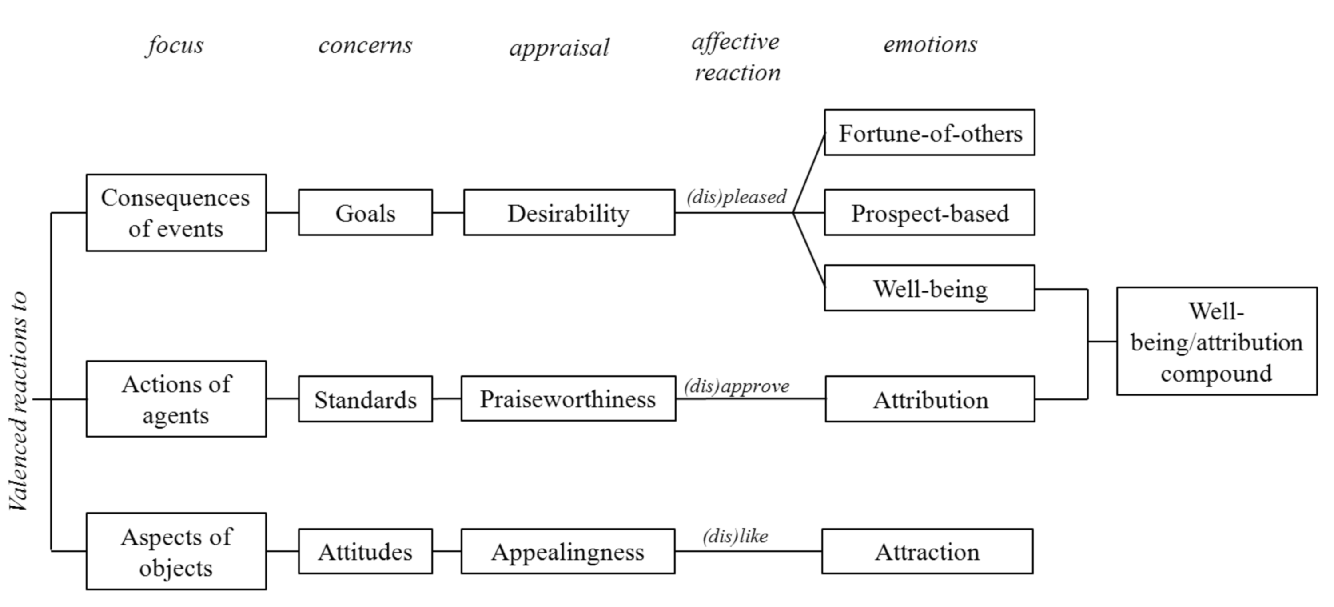
\includegraphics[width=\textwidth]{figure/occ.png}
  \caption{A simple visualization of OCC model \cite{occ:structure}.}
  \label{fig:occ-model}
\end{figure}

As shown in Figure \ref{fig:occ-model}, a person could alternatively have three
types of focuses. These types of focuses are consequence of events, actions of
agents, and aspects of objects. The person evaluates the significance of causes
behind these three types of focuses based on her personal concern. As a
result, an affective reaction will be elicited resulting in an emotion. Various
combinations of the elements depicted in Figure \ref{fig:occ-model} create
specific patterns demonstrating six main groups of emotions in which all emotion
types in a group share the same cognitive pattern. Emotion groups are
\textit{fortune-of-others, prospect-based, well-being, attribution,
well-being/attribution- compound}, and \textit{attraction}. The OCC model
introduces 22 emotion types. These emotions are introduced each as a
representative of a family of similar emotions with various intensities
(since relying on a list of discrete emotions that is understood by everyone
equally is impossible due to people's language barriers and various
interpretations of the actual words). For instance, happiness can be referred
to by other emotion terms such as joy, cheerfulness, gladness, delighted while
they all share the same eliciting conditions. Thus the emotion types used in the
model (e.g., relief, love, pride, and shame) are meant to represent an emotional
experience rather than a lexical taxonomy.

For instance, as shown in Figure \ref{fig:occ-model}, the appraisal criterion
for consequences of event’s is their \textit{desirability} (see Section
\ref{sec:appraisal-theory}) for achieving one's goals. This generates the
affective reaction of being \textit{pleased} in positive cases, or
\textit{displeased} in negative ones. Figure \ref{fig:occ-structure} shows the
resulting emotion groups in OCC model such as \textit{fortune-of-others} (e.g.,
gloating, pity), \textit{prospect- based} (e.g., satisfaction, relief), and
\textit{well-being} (e.g., joy, distress) \cite{occ:structure}. The appraisal of
the praiseworthiness of the actions of an agent against one's personal
standards, as well as the appealing aspects of objects happens in the same way
as shown in Figure \ref{fig:occ-model}.

\begin{figure}[tbh]
  \center
  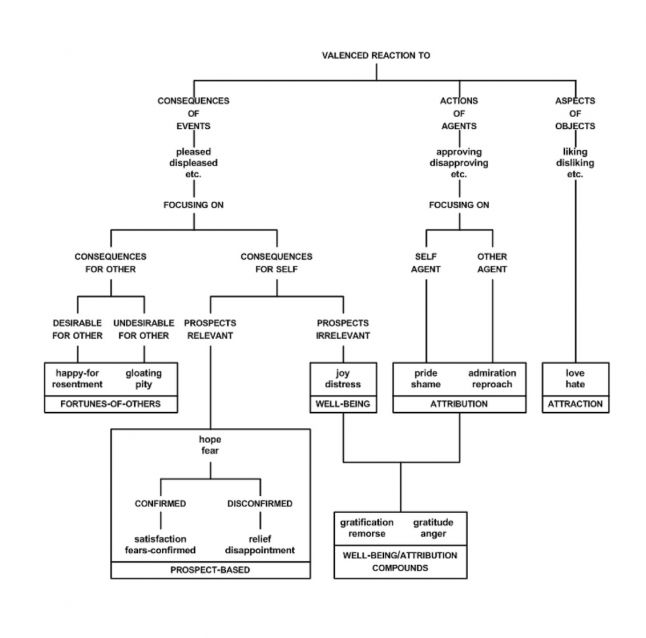
\includegraphics[width=0.9\textwidth]{figure/occ-structure.jpg}
  \caption{OCC taxonomy of emotion triggers and emotions \cite{occ:structure}.}
  \label{fig:occ-structure}
\end{figure}

Finally, the OCC model introduces some global variables of an emotion's
intensity to distinguish all types of emotions that a person could experience when
encountering events, agents or objects. These variables are as follows:

\begin{enumerate}
	\item Sense of reality (representing the degree to which the event, agent or
	object in focus appear real to the person),

	\item Proximity variable (representing the psychological proximity of an event,
	agent or object),

	\item Unexpectedness (representing how surprising an event is for one, either
	positive or negative),

	\item Arousal (representing how arousing an event, agent or object is).
\end{enumerate}

\subsection{Constructivist (Dimensional) Emotion Theories}
\label{sec:dimensional-emotions}

The components and dimensions of emotions were the subject of much speculation
since the 19th century. Dimensional models of emotion attempt to conceptualize
human emotions by defining where they lie in two or three dimensions.
Dimensional theories of emotion argue that emotion should be conceptualized, as
points in a continuous (typically two or three) dimensional space rather than
looking at them as discrete entities (see Section \ref{sec:discrete-emotions})
\cite{carver:affect-behavior} \cite{mehrabian-russell:pad}
\cite{russell:core-affect} \cite{watson:consensual-structure-mood}. 

\begin{figure}[tbh]
  \center
  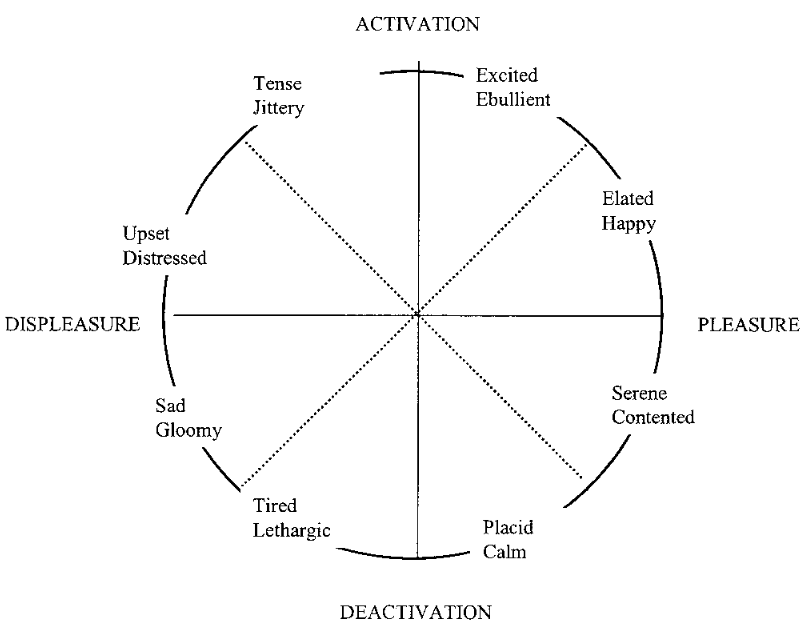
\includegraphics[width=.7\textwidth]{figure/core-affect.png}
  \caption{Russell's suggested affective states based on core affect
  \cite{russell:core-affect}.}
  \label{fig:core-affect}
\end{figure}

Two dimensions that are commonly proposed to describe emotions are valence and
physiological arousal \cite{arnold:emotion-personality}
\cite{lazarus:cognitive-theory-emotion} \cite{russell:circumplex-affect}. Models
based on dimensional theories contrast theories of basic emotion, which propose
that different emotions arise from separate neural systems
\cite{posner:circumplex-affect}. Many dimensional theories argue that discrete
emotion categories (e.g., sadness, fear and anger) have no ``reality'' in that
there are no specific brain regions or functions that correspond to specific
emotions \cite{barrett:emotions-natural}. Dimensional theories do not emphasize
the term emotion.

\begin{figure}[tbh]
  \center
  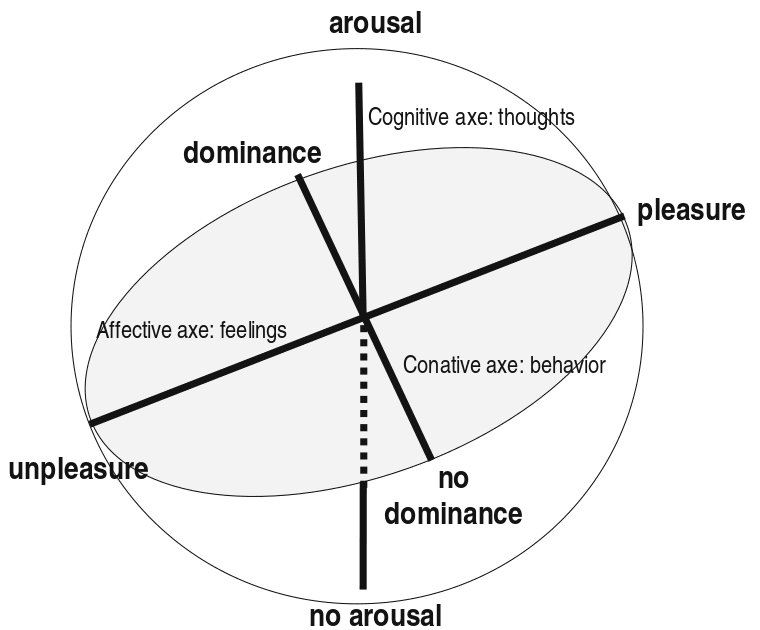
\includegraphics[width=.6\textwidth]{figure/dimensional2.png}
  \caption{Three dimensional model of pleasure, arousal and dominance as
  tripartite view of experience \cite{mehrabian:pad}.}
  \label{fig:pad}
\end{figure}

One of the most prominent two-dimensional models is Russell's circumplex model
\cite{russell:circumplex-affect}. Russell suggested that affective states are
all related to each other systematically through what is called core affect
\cite{russell:circumplex-affect,russell:core-affect} (see Figure
\ref{fig:core-affect}) and emotions are best described as a change in core
affect which, in turn, is describable as a point in a space between two bipolar
dimensions. One dimension is \textit{valence} or how good or bad objects and
events are for a being ranging from pleasant to unpleasant. The other dimension
is \textit{arousal}, ranging from calm to excited. Russell put a number of
affective states around a circular space between those two dimensions (see
Figure \ref{fig:core-affect}) which is also known as \textit{circumplex},
representing the variety of core affects
\cite{russell:circumplex-affect,russell:core-affect}. Since sometimes
two-dimensional space cannot easily differentiate among emotions that share the
same values of arousal and valence, e.g., anger and fear (both characterized by
high arousal and negative valence), some of the dimensional models incorporate
valence and arousal as well as \textit{intensity}, or \textit{dominance} or
\textit{stance} dimensions. Many computational dimensional models build on the
three dimensional “PAD” model of Mehrabian and Russell
\cite{mehrabian-russell:pad} where these dimensions correspond to pleasure (a
measure of valence), arousal (indicating the level of affective activation) and
dominance (a measure of power or control). Figure \ref{fig:pad} shows these
three dimensions.

\begin{figure}[tbh]
  \center
  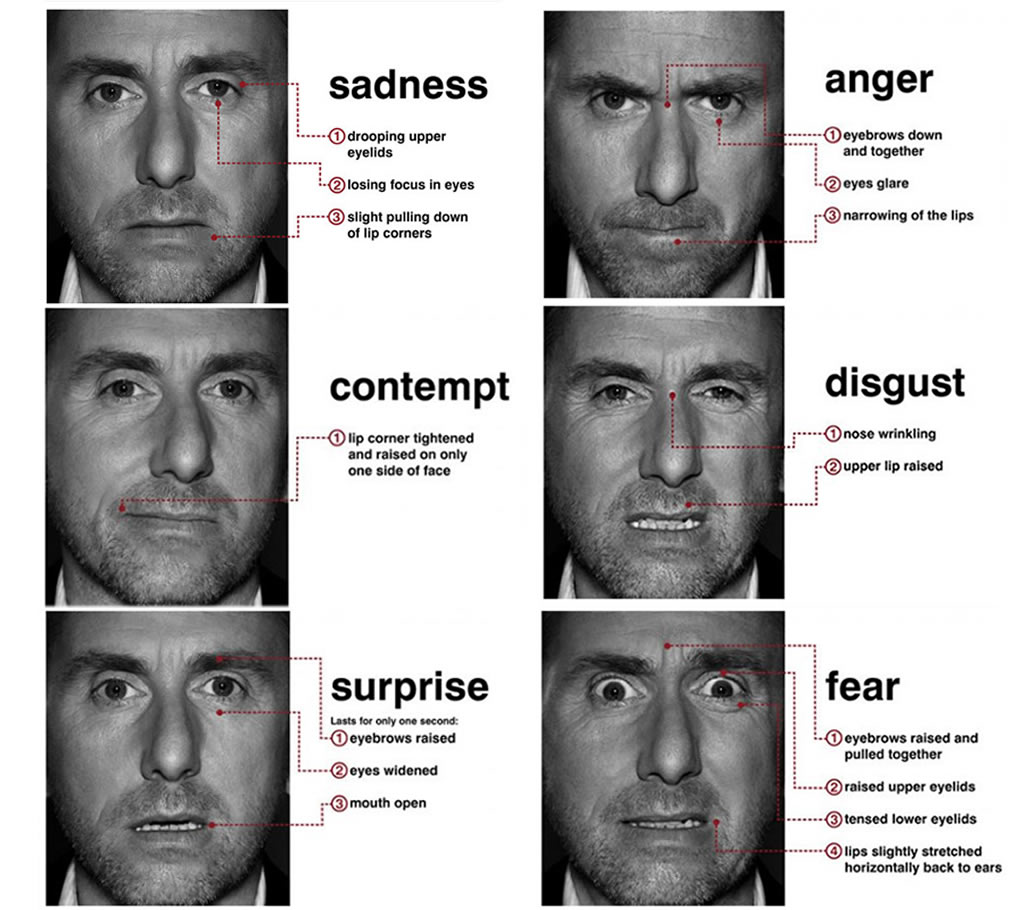
\includegraphics[width=.9\textwidth]{figure/basic-emotions.jpg}
  \caption{Basic emotions and corresponding expressions.}
  \label{fig:basic-emotions}
\end{figure}

\subsection{Basic (Discrete) Emotion Theories}
\label{sec:discrete-emotions}

Basic emotion theories are inspired by Tomkins' \cite{tomkins:affect}
rediscovery of Darwin's work
\cite{darwin:emotion-expression,hess:darwin-emotion} which later were developed
by Ekman \cite{ekman:argument-emotions} and Izard \cite{izard:human-emotions}.
These theories emphasize a small set of discrete and fundamental emotions.
The underlying assumption of this approach is that these emotions are mediated
by associated neural circuitry, with a hardwired component
\cite{ekman:argument-emotions}. Different emotions are then characterized by
stable patterns of triggers, behavioral expression, and associated distinct
subjective experiences. The emotions addressed by these theories are typically
called the \textit{basic} emotions. Emotions including happiness, sadness, fear,
anger, surprise, and disgust are often considered to comprise the most
prototypical basic emotions \cite{ekman:argument-emotions}. The theory of basic
emotions holds that there is a set of emotions shared by all humans that evolved
to deal with ancestral life challenges \cite{ekman:argument-emotions}. For
instance, disgust evolved to deal with the challenge of avoiding noxious
stimuli, and fear evolved to deal with the challenge of avoiding dangers.
Because of the emphasis on discrete categories of states, this approach is also
termed the \textit{categorical} approach \cite{panskepp:affective-neuroscience}.
Much of the supporting evidence offered for the theory comes from experiments
that show how certain facial expressions are universally associated with
specific basic emotions, regardless of the observer's cultural background. This
universality has a production side and a recognition side. On the production
side, a particular emotional state is said to elicit a facial expression
comprised of a fixed set of facial muscles. On the recognition side, observers
are able to infer the emotional state of the person who expresses an emotion,
due to the direct correspondence between emotional states and the facial
expressions they cause. Computational models inspired by the basic emotions or
discrete approach often focus on low-level perceptual-motor tasks and encode a
two-process view of emotion that argues for a fast, automatic, undifferentiated
emotional response and a slower, more differentiated response that relies on
higher level reasoning processes (e.g.,
\cite{armony:computational-modeling-emotion}).

\subsection{Other Approaches}

There are other approaches that different researchers take based on their
emphasis on the applicability of emotions in their systems.

\subsubsection{Rational Approaches}

Rational approaches start from the question of what adaptive functions emotions
serve and then attempt to incorporate these functions into a model of
intelligence. Emotion, within this approach, is simply another set of processes
and constraints that have adaptive value. Models of this sort are most naturally
directed towards the goal of improving theories of machine intelligence
\cite{anderson:newell-cognition} \cite{scheutz:affect-agent}
\cite{simon:motivation-emotion-cognition}.

\subsubsection{Communicative Approaches}

Communicative theories of emotion argue that emotion processes function as a
communicative system. They can function first, as a mechanism for informing
other individuals of one’s mental state (thereby facilitating social
coordination), and second, as a mechanism for requesting/demanding changes in
the behavior of others. Communicative theories emphasize the
social-communicative function of expressions \cite{gratch:emotion-intention}.
Computational models inspired by communicative theories focus on machinery that
decides when an emotional expression can have a desirable effect on a human
counterpart.

\section{Similarities and Differences}
\label{sec:comparison}

Different theoretical perspectives should not be viewed as competing for a
single truth. They should be seen as distinct perspectives, each arising from a
particular research area (e.g., biological vs. social psychology), focusing on
different sets of affective phenomena, considering distinct levels of resolution
and fundamental components (e.g., emotions vs. appraisal variables as the
distinct primitives). These different perspectives also provide different
degrees of support for the distinct processes of emotion, e.g., the componential
theories provide extensive details about cognitive appraisals
\cite{hudlicka:guidelines-emotions}. Therefore, I am going to provide a pairwise
comparison between these fundamental theories. Note that a distinct pairwise
comparison will not be provided for appraisal vs.\,discrete (basic) emotion
theories as important points are adequately covered in the comparisons presented
below.

\subsection{Dimensional Vs. Discrete (Basic) Emotion Theories}

The fundamental assumption of the basic emotion theory is that a specific type
of event triggers a specific affect program corresponding to one of the basic
emotions and producing characteristic expression patterns and physiological
response configurations \cite{scherer:emotions-emergent}. Dimensional theory's
main criticism of basic emotions theory is based on the observation that
affective phenomena appear to be both qualitatively and quantitatively diverse.

Russell in \cite{russell:core-affect} argues the labels such as ``fear",
``anger'', ``happiness'' do not capture this diversity. For instance, one might
say: a) a person being chased by an assailant brandishing a knife, b) a person
who retreats from an insect moving across the floor, and c) a person who is
concerned they will never find a fulfilling career are all in a state of
fear. On the basic emotions account, an emotional episode involves fixed
patterns of neurophysiological and facial expression changes in response to an
eliciting stimulus that are distinct between emotions, but are the same within
the same emotional category \cite{ekman:argument-emotions}. If this were the
case, one would expect that the three individuals described above would respond
to their eliciting stimuli in the same way, yet the similarity of behavioral
responses between these three cases seem unlikely. Dimensional theorists, in
contrast, would argue that the individuals in the above three cases are applying
the concept of fear to experience, despite the fact that each individual has a
unique core affect. While basic emotion theorists would hold that since all
three individuals are experiencing fear, they would perform the same behavioral
responses to the stimuli, dimensional theorists would argue this is not the
case, as each individual bears a core affective state that is distinguished from
the other two. For instance, the individual's arousal in response to an armed
assailant should be higher than the individual in response to an insect, as the
former case poses a threat to their life. As a result, the individual in the
first case would likely make every effort to escape from the assailant,
including trying to negotiate and plead with the assailant, while the individual
in the second case would be relatively less dedicated to escaping the insect. 

In sum, dimensional theory is compatible with the differences in the behavioral
responses to eliciting stimuli, while basic emotions theory only allows for a
single fixed behavior of responses to a given emotion. Furthermore, dimensional
theories can represent instances of basic emotions (see Figure
\ref{fig:dimensional-discrete}), for example, fear elicited by a snake (green
rectangle), in terms of variation along affective dimensions, i.e., arousal and
valence.

\begin{figure}[tbh]
  \center
  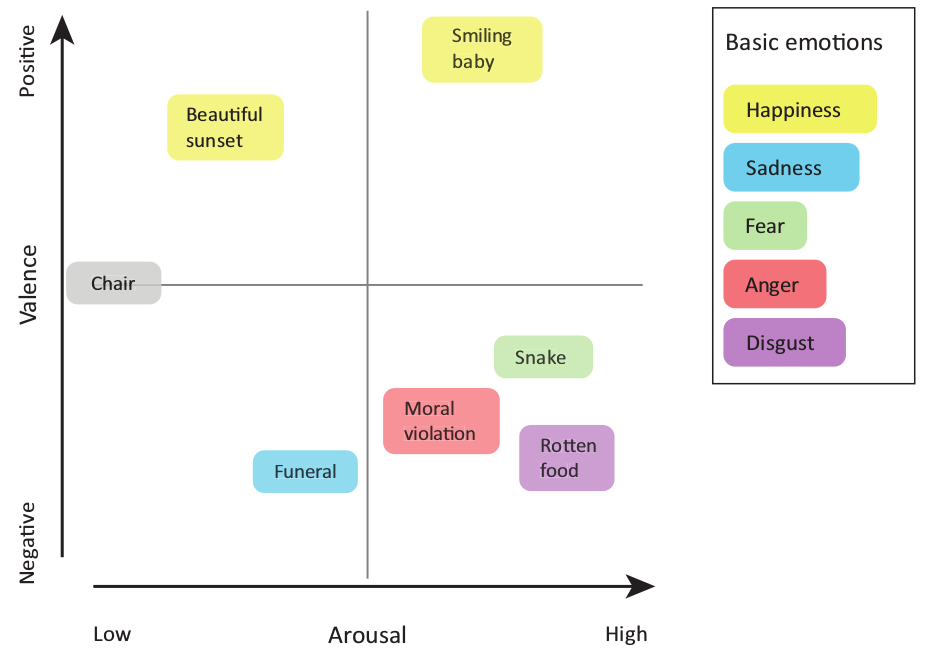
\includegraphics[width=.9\textwidth]{figure/dimensional-discrete.png}
  \caption{Representing basic emotions within a dimensional framework
  \cite{hamann:mapping-discrete-dimensional}.}
  \label{fig:dimensional-discrete}
\end{figure}

Also, basic emotion theory fails to account for affect that lacks
object-directedness \cite{russell:core-affect}. In basic emotions approach, an
emotion is supposed to have an intentional object it is directed towards (e.g.,
being angry at someone, or being sad for someone). The dimensional theory argues
that emotion may not necessarily be aimed at a particular object. For instance,
an individual can experience a certain type of emotion (e.g., anger) without
knowing of anything in particular that has offended her. Dimensional models of
emotion are therefore capable of accounting for a wider range of affective
phenomena than basic emotions theory.

Another difference between dimensional and basic emotion theories is that the
basic emotion categorization of emotions captures facets of the experience of
an emotion not conveyed by the dimensional description, such as elicitation of a
facial expression of the emotion. In fact, this attribute of the basic
emotions theory is one of the major differences with all other emotion theories.
As it is argued in basic emotion theory, basic emotions are hard-wired to their
corresponding facial expressions. Ekman who elaborated the concept of basic
emotions, developed the \textit{Facial Action Coding System} (FACS) which
encodes movements of individual facial muscles and it is a common standard to
systematically categorize the physical expression of emotions
\cite{ekman:facial-movement}.

\subsection{Appraisal Vs. Dimensional Emotions Theories}

Dimensional theories might struggle to adequately distinguish emotions because
of the existence of limited dimensions.

To compare the appraisal and dimensional theories of emotion, we can argue that
there is a relationship between the dimensions in the constructivist or
dimensional theory of emotion and appraisal dimensions. For instance, the
pleasure dimension roughly maps onto appraisal dimensions that characterize the
valence of an appraisal-eliciting event (e.g., intrinsic pleasantness
--desirability--, or goal congruence), dominance roughly maps onto the appraisal
dimension of coping potential, and arousal can be considered as a measure of
intensity. However, they also have quite different meanings. Appraisal (as I
mentioned earlier) is a relational construct characterizing the relationship
between some specific object/event in the environment and the individual's
mental constructs including beliefs, motives and intentions and several
appraisals may be simultaneously active; whereas emotions in dimensional emotion
theory are non-relational constructs, each summarizing a unique overall state of
the individual.

Furthermore, dimensional emotion theories emphasize different components of
emotion than appraisal theories and link these components quite differently.
In contrast to appraisal theories, dimensional emotion theories do not address
affect’s antecedents in detail. However, dimensional theorists question the
tight causal linkage between appraisal and emotion that is central to appraisal
accounts. As mentioned earlier, dimensional theorists believe that the emotion
is not necessarily about some object (as in ``I am angry \underline{at him}'').
In such theories, many factors may contribute to a change in emotion including
intentional judgments (e.g., appraisal). However, in dimensional emotion
theories the link between any preceding intentional meaning and emotion is
broken and most of the time can not be recovered correctly. For example, Russell
argues for the following sequence of emotional components: some external event
occurs (e.g., a bear walks out of the forest), it is perceived in terms of its
affective quality; this perception results in a crucial change in core affect;
this change is attributed to some ``object" (e.g., the bear); and only then is
the object cognitively appraised in terms of its goal relevance, causal
antecedents and future prospects \cite{marsella:computational-models}.

We can also compare the dimensional emotion theories to OCC model as a cognitive
appraisal model. The major similarity between these two models is that they both
consider emotions to descend from valenced reactions to the stimuli.
Furthermore, they acknowledge the role of arousal in determining emotional
reactions. As we mentioned in Section \ref{sec:dimensional-emotions} Russell
considered arousal as one of the two key dimensions of emotions which could be
used to partially discriminate emotional states
\cite{russell:circumplex-affect}. In a different manner, the OCC model
recognizes arousal as a necessary condition for eliciting emotions, and regards
the arousal as a major determinant of the elicited emotion's intensity which
distinguishes among various emotions of a particular type (e.g., fearful and
scared). In \cite{scherer:what-emotions} Scherer speculates that the arousal
dimension in dimensional models gives little information about the underlying
appraisal of the elicited emotion and he proposes to replace it with coping
potential which is an appraisal dimension referring to the individual's
perceived control in a given situation.

Furthermore, models based on dimensional emotions theory pursue the idea of
eliciting an emotion according to the joint features in circumplex space (2D or
3D -- see Section \ref{sec:dimensional-emotions}) while OCC or other
models of appraisal theory are based on patterns of antecedents of emotions.
This is the fundamental difference between OCC, or appraisal theories in
general, and the circumplex approach of Russell \cite{russell:circumplex-affect}
or Mehrabian's PAD model \cite{mehrabian:pad,mehrabian-russell:pad}. Also,
models based on appraisal theory of emotion employ causation, attribution and
eliciting conditions in order to distinguish emotions while the eliciting
conditions are not directly accessible from dimensional approach. A dimensional
model might fall short in establishing why certain emotions are elicited.
However, when the objective is to identify the generated emotions and their
level of pleasantness and intensity, a circumplex model presents a perfect
opportunity \cite{ahmadpour:occ-dimensional-comparison}.

\begin{figure}[tbh]
  \center
  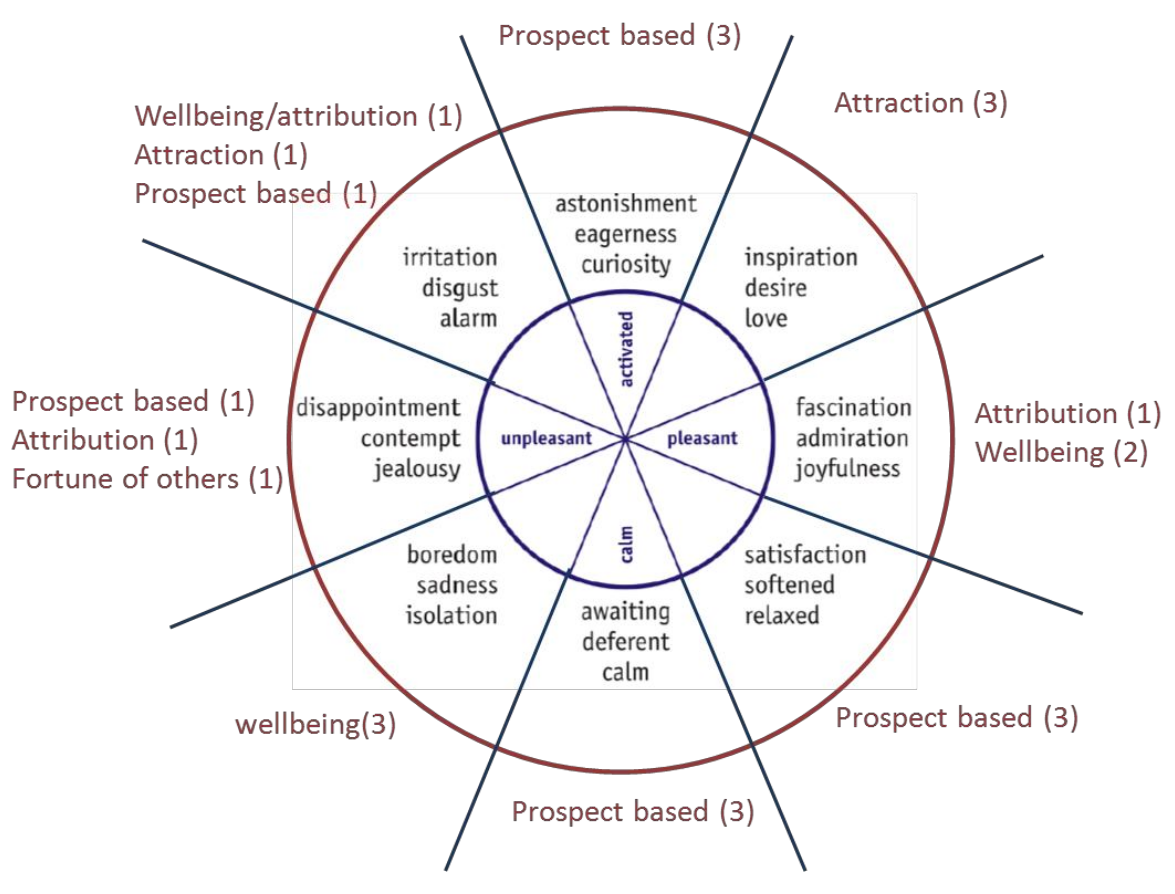
\includegraphics[width=.9\textwidth]{figure/occ-circumplex-mapping.png}
  \caption{A rough projection of emotion groups of OCC on the circumplex of
  affect \cite{ahmadpour:occ-dimensional-comparison}.}
  \label{fig:occ-circumplex}
\end{figure}

Finally, here, I discuss how a model based on dimensional emotions theory
(i.e., Russell's 2D circumplex) relates to a cognitive model based on appraisal
theory (i.e., OCC model). Figure \ref{fig:occ-circumplex} shows the relationship
between Russell's circumplex and OCC model in terms of categorization of the
actual emotions. The number of emotions in a section of Russell's circumplex
that fall into an emotion group of OCC are shown in parentheses (see Figure
\ref{fig:occ-circumplex}). For instance, all three emotions in the top section
(highly excited, neutrally valenced emotions) fall into prospect based emotion
group, hence number (3) is indicated. Or, as another example, emotions in the
left section (neutral arousal value, negative valenced emotions) make a one to
one relationship between disappointment and prospect based emotion group,
contempt and attribution emotion group, and jealousy and fortune of others
emotion group, hence number (1) is indicated in front of each.

\section{Applications in Autonomous Agents and Robots}
\label{sec:applications}

There are many research areas, including robotics and autonomous agents, that
employ the structure and/or functions of emotions in their work with a variety
of motivations behind modeling emotions
\cite{wehrle:motivations-modeling-emotion}. Some of these works are inspired by
specific psychological theories (we provide several examples in this section),
some are freely using the concept of emotion without using the theoretical
background in social sciences, and some are using a combination of concepts from
the psychological theories. For instance, in PECS \cite{urban:pecs} which is
designed for modeling human behaviors, the agent's architecture is not based on
a certain kind of social or psychological emotion theory. In fact, it is
intentionally designed and described in a way which enables the integration of a
variety of theories. The PECS' design enables an integrative modeling of
physical, emotional, cognitive and social influences within a component-oriented
agent architecture. Also, in \cite{miranda:teamwork-multiagent-system} the
computational architecture which is designed to provide information about the
possible overall behavior of a work team is not based any specific theory. As
we mentioned earlier, some researchers apply combinations of emotion theories in
their work \cite{kiryazov:modeling-appraisal-pad}. For instance, in
\cite{canamero:designing-activity-selection} Ca$\tilde{n}$amero shows how an
agent can use emotions for activity selection while taking into account both
dimensional and discrete approaches in an action selection mechanism. Through
out this section, we provide different examples of works using major emotion
theories in robots and autonomous agents.

We can also see the application of emotion theories in designing companion
robots, robots capable of expressing emotions and social behaviors, as well
as robots which can convey certain types of emotion products, e.g., empathy
\cite{breazeal:expressive-behavior} \cite{leite:empathy-hri}
\cite{paiva:emotion-modeling} \cite{shayganfar:methodology}. Robots also use
emotions theories for automatic affect recognition using different modalities
\cite{hegel:empathic-robot} \cite{zeng:affect-recognition}. Moreover, in some
works, researchers have explored the user’s affective state as a mechanism to
adapt the robot's behaviors during the interaction
\cite{breazeal:sociable-robot} \cite{liu:affect-robot-behavior}.\\

\textbf{Applications of Appraisal Theory} -- The emphasis of models derived from
appraisal theories of emotion is on making appraisal the central process.
Computational appraisal models often exploit elaborate mechanisms for deriving
appraisal variables such as decision-theoretic plans
\cite{gratch:domain-independent} \cite{marsella:ema-process-model}, reactive
plans \cite{rank:appraisal-story-world} \cite{neal:modeling-antecedents}
\cite{staller:emotion-social-norm}, Markov-decision processes
\cite{elnasr:flame} \cite{si:modeling-appraisal-tom-journal}, or detailed
cognitive models \cite{marinier:behavior-emotion}. However, emotion itself is
sometimes treated less elaborately, and simply as a label to which behavior can
be attached \cite{elliott:affective-reasoner}. Appraisal is usually modeled as
the cause of emotion being derived via simple rules on a set of appraisal
variables.

Computational appraisal models have been applied to a variety of uses including
contributions to psychology, robotics, AI, and HCI. For instance, Marsella and
Gratch have used EMA \cite{marsella:ema-process-model} to generate specific
predictions about how human subjects will appraise and cope with emotional
situations and argue that empirical tests of these predictions have implications
for psychological appraisal theory \cite{gratch:assessing-appraisal}
\cite{marsella:assessing-coping}. There are several examples in artificial
intelligence and robotics of applying appraisal theory
\cite{adam:bdi-emotional-companion} \cite{kim:model-hri-appraisal}
\cite{marsella:ema-process-model}. In robotics, appraisal theory has been used
to establish and maintain a better interaction between a robot and a human. For
instance in \cite{kim:model-hri-appraisal} researchers provide their
computational model of emotion generation based on appraisal theory to have a
positive human-robot interaction experience. In
\cite{sander:systems-approach-appraisal} authors describe a system approach to
appraisal processes based on Scherer's work on appraisal and the Component
Process Model \cite{scherer:nature-function-emotion}. They show how the
temporal unfolding of emotions can be experimentally tested. They also lay out a
general domain-independent computational model of appraisal and coping. In
\cite{vogiatzis:robot-museum} researchers consider their robot's (INDIGO)
emotion, speech and facial expressions as a key point to establish an effective
communication between the robot and a human during their interaction. They apply
concepts of appraisal theory in INDIGO's emotion modeling. MAGGIE, a sociable
robot, also applies the appraisal theory of emotions to consider fear in its
decision making system \cite{castro:autonomous-robot-fear}. Velasquez developed
Cathexis which is a distributed computational model for generation of emotions
and their influence in the behavior of the autonomous agents
\cite{velasquez:emotions-motivations-agents}. The emotion model in this work is
based on Roseman's work on appraisal theory. Marinier and Laird in
\cite{marinier:emotion-reinforcement} focus on the functional benefits of
emotion in a cognitive system. In this work, they integrate their emotion theory
(which is based on the appraisal theory) with Soar cognitive architecture, and
use emotional feedback to drive reinforcement learning. In
\cite{hudlicka:emotinos-reasons} Hudlicka provides a model of a generic
mechanism mediating the affective influences on cognition based on cognitive
appraisal. This model is implemented within a domain-independent
cognitive-affective architecture (MAMAID). 

In the virtual agents community, empathy is a research topic that has received
much attention in the last decade \cite{brave:emotion-hci}
\cite{scott:modeling-empathy-agent} \cite{paiva:agent-care}
\cite{prendinger:empathic-companion} \cite{bickmore:longterm-relationship}. In
\cite{pontier:women-robot-men} researchers developed an agent with capability of
affective decision-making based on appraisal theory to establish an affective
relationship with its users. Then, they compared the performance of their agent
with a human (based on a WoZ study) in a speed-dating experiment. In HCI, the
appraisal theory has been primarily used for the creation of interactive
characters that exhibit emotions in order to make characters more believable
\cite{neal:believable-agents}, more realistic \cite{mao:social-causality}
\cite{traum:negotiation-teams-training}, more capable of understanding human
motivational states \cite{conati:evaluating-student-affect} or more able to
induce desirable social effects in human users \cite{paiva:learning-feeling}.

\textbf{Applications of Dimensional Theory} -- The emphasis of models influenced
by dimensional theories is on processes associated with core affect which is
usually represented as a continuous time-varying process, and it can be
determined at a given time by a point in a 2D or 3D-space as a response to the
eliciting events. Generally, there are detailed mechanisms in computational
dimensional models which determine how this point changes over time, e.g., decay
to some resting state, and incorporating the impact of dispositional tendencies
such as personality or temperament \cite{gebhard:alma}
\cite{marsella:computational-models}. The models based on dimensional theories
have also been used in robotics. For instance, researchers in
\cite{lim:mei-motherese-ei} apply PAD's three-dimensional space to rate the
pleasure, arousal and dominance of their Multimodal Emotional Intelligence robot
(MEI) in each interaction with human subjects. Their goal is to introduce the
first steps in MEI which can understand and express emotions in voice, gesture
and gait. In \cite{zhang:service-robot-dimensional} researchers want to
understand the effect of different interface features for a service robot. They
use valence and arousal dimensions in their questionnaires to assess the
perceived anthropomorphism of their own service robot by their subjects. In
\cite{klug:emotion-based-hri} researchers introduce the implementation of a
dynamic personality for a robot based on a dimensional emotion model. They use
WASABI's architecture \cite{becker:wasabi,becker:wasabi-description} as their
emotional model. In \cite{lisetti:affect-socially-intelligent} the author
describes an affective knowledge representation scheme to be used in the design
of a socially intelligent artificial agent. Lisetti uses the valence-arousal two
dimensional model of emotion in this work. This model has been applied in an
emotion-based architecture of Lisetti's autonomous robots as well as a
multimodal affective user interface agent. ROMAN, an expressive robotic head,
uses a behavior-based emotional control architecture. The approach to the
emotional component of the architecture is based on the dimensional emotion
theory \cite{hirth:roman}.

\textbf{Comparison of Applications of Emotion Theories} -- Researchers often use
computational dimensional models for behavior generation of animated characters.
The reason might be because it is easier for emotion translation to a limited
number of dimensions that can be readily mapped to continuous features of
behavior such as the spatial extent of a facial expression. For example, PAD
models describe all behavior in terms of only three dimensions of pleasure,
arousal and dominance, whereas researchers using appraisal models should either
associate each behavior with a large number of appraisal variables
\cite{scherer:expression-appraisal}
\cite{smith:computational-facial-expression}, or try to map appraisal variables
into a limited and small number of discrete expressions
\cite{elliott:affective-reasoner}. For a similar reason, dimensional models also
frequently used as a good representational framework for systems that attempt to
recognize human emotional behavior and there is some evidence that they may
better discriminate user affective states than approaches that rely on discrete
labels \cite{barrett:emotions-natural}.

There is also a relationship between dimensional and appraisal theories. Some of
the computational models of emotion that incorporate dimensional theories have
viewed appraisal as the mechanism that initiates changes to core affect. For
instance, ALMA \cite{gebhard:alma} includes OCC inspired appraisal rules
\cite{occ:structure}, and WASABI \cite{becker:wasabi} includes appraisal
processes inspired by Scherer's sequential-checking theory into a PAD-based
emotion model. Moreover, some computational models explore how core affect in
dimensional models can influence cognitive processes. For example, HOTCO 2
\cite{thagard:emotional-coherence} allows explanations to be biased by
dimensional affect \cite{marsella:computational-models}.

\section{Conclusion}
\label{sec:conclusion}

In this response, we started by looking at the description of affective
computing and the importance of the concept of emotion in general. Then, we
provided our four categories of computational models of emotions which we can
consider for the applications of affective computing.

There are major theories of emotions explaining the concept of emotion. We
discussed these major theories in detail separately, providing their
psychological background and underlying concepts. Following the explanation of
these theories, we were able to discuss the similarities and differences between
these major theories. Finally, we provided applications of these theories in
robotics and AI.

We believe to develop or work based on computational models of emotions, it is
good to follow well-established (in comparison with others) theoretical
foundations. These theories can be a guideline for our computational models, and
they can explain more details of the structure or the processes involved in
affective situations. However, we do not necessarily think that the
computational models must exactly follow only one theory and its descriptions.
Meaning, different aspects of models can represent different theories. For
instance, appraisal theory is a good representation of the interpretive aspect
of emotions and basic emotion theories provide detailed systematic methods for
expressive application. More importantly, we believe the interpersonal functions
of emotions should be our first concern and try to relate them to the structure
of our domain, i.e., collaboration. In conclusion, we can see the importance of
interpretive, communicative and regulatory aspects of emotion functions in this
proposed work.

\bibliographystyle{plain}
\bibliography{mshayganfar}

\end{document}

















